\subsection{Die Klausur}

\subsubsection*{Aufgabe: Entscheidungen unter Unwissenheit}

%\begin{enumerate}

%\item 
% Geben Sie an, welche der drei Handlungen $A_1$, $A_2$ oder $A_3$
% nach der {\em Maximin-Regel} gewählt werden sollte:
% \begin{center}
% \begin{tabular}{c|c|c|c|}
% \multicolumn{1}{c}{} & \multicolumn{1}{c}{$S_1$}
% & \multicolumn{1}{c}{$S_2$} & \multicolumn{1}{c}{$S_3$} 
% \\ \cline{2-4}
% $A_1$ & 1 & -1 &  5 \\ \cline{2-4} 
% $A_2$ & 3 &  7 & -2 \\ \cline{2-4}
% $A_3$ & 4 & -1 &  1 \\ \cline{2-4}
% \end{tabular}
% \end{center}

%\item 
Lösen Sie nach der Minimax-Bedauerns-Regel. Stellen Sie dazu die
Bedauernstabelle auf und geben Sie dann an, welche drei Handlungen $A_1$, $A_2$
oder $A_3$ gewählt werden sollte.
\begin{center}
\begin{tabular}{c|c|c|c|c|}
\multicolumn{1}{c}{} & \multicolumn{1}{c}{$S_1$}
& \multicolumn{1}{c}{$S_2$} & \multicolumn{1}{c}{$S_3$}
& \multicolumn{1}{c}{$S_4$}
\\ \cline{2-5}
$A_1$ &   3 &   7  &  500 &  4 \\ \cline{2-5} 
$A_2$ & 200 &  100 &    3 & 50 \\ \cline{2-5}
$A_3$ & 150 &   60 &    2 & 25 \\ \cline{2-5}
\end{tabular}
\end{center}

%\end{enumerate}

\subsubsection*{Aufgabe: Entscheidungsbäume}
\label{BaumAufgabe}
Eine Person steht vor einem Entscheidungsproblem, das durch den Entscheidungsbaum {\em auf der letzten Seite} dargestellt wird:
%\begin{center}
%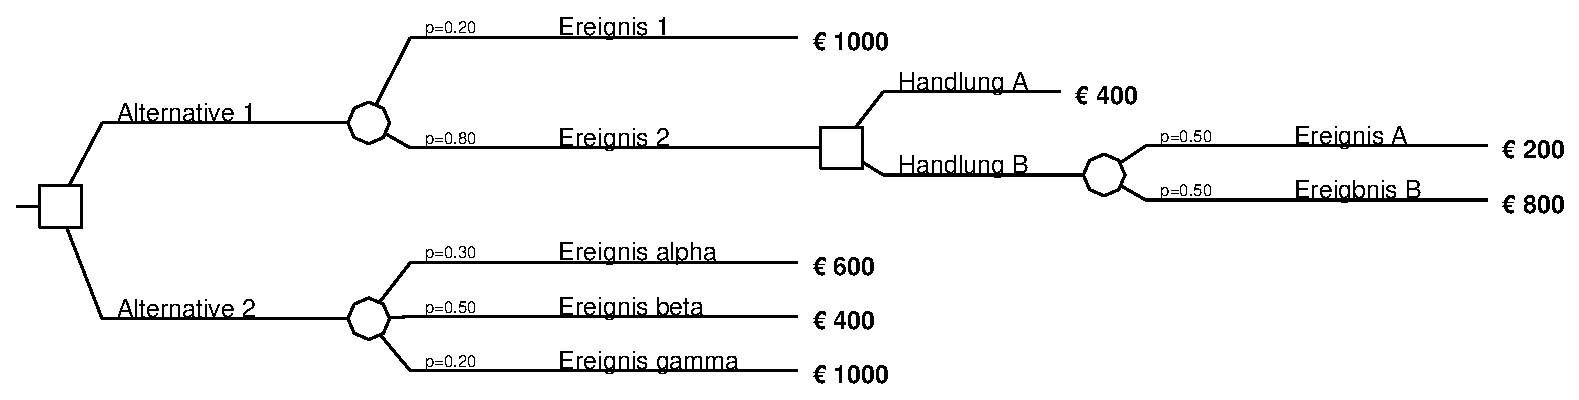
\includegraphics[width=12.5cm]{Grafiken/Klausur.ps}
%\end{center} 
\begin{enumerate}
  \item Sollte die Person an dem weiter rechts liegenden der beiden
  Entscheidungsknoten besser "`Handlung A"' oder "`Handlung B"' wählen?
  \item Wie groß ist der Erwartungswert von "`Alternative 1"' (am ersten
  Entscheidungsknoten von links)?
  \item Sollte die Person "`Alternative 1"' oder "`Alternative 2"' wählen?
\end{enumerate}
(Nehmen Sie dabei an, dass die Person sich rational verhält und den Wert von
zufälligen Ereignissen immer nach dem Erwartungsnutzenprinzip berechnet.)

\subsubsection*{Aufgabe: Nash-Gleichgewichte}

Gegeben sei folgendes Zwei-Personen Spiel:

\begin{center}
\begin{tabular}{c|c|c|}
\multicolumn{1}{c}{} & \multicolumn{1}{c}{$S_1$} &
                               \multicolumn{1}{c}{$S_2$} \\ \cline{2-3} 
$Z_1$                & 1, 1           & 2, 0  \\ \cline{2-3} 
$Z_2$                & 0, 2           & 4, 4  \\ \cline{2-3}
\end{tabular}
\end{center}

\begin{enumerate}
  \item Geben Sie alle {\em reinen} Nash-Gleichgewichte des Spiels an.
  \item Berechnen Sie das {\em gemischte} Nash-Gleichgewicht. Geben Sie an, mit
  welcher Wahrscheinlichkeit der Zeilenspieler im gemischten Gleichgewicht $Z_1$ spielt, und mit welcher 
  Wahrscheinlichkeit der Spaltenspieler im gemischten Gleichgewicht $S_1$ spielt.
\end{enumerate}


\subsubsection*{Aufgabe: Bayes'scher Lehrsatz}

Ein Bergbau-Unternehmen möchte in Sibieren Gold abbauen. Experten schätzen,
dass in dem dafür vorgesehenen Gebiet mit einer Wahrscheinlichkeit von {\bf
30\%} reiche Goldvorkommen zu finden sind. Bevor das Unternehmen jedoch eine
Abbau-Konzession von der Regierung erwirbt, hat es sich das Recht vorbehalten,
Probegrabungen durchzuführen. Falls tatsächlich Goldvorkommen vorhanden
sind, dann liefern die Probegrabungen mit {\bf 95\%} Wahrscheinlichkeit 
ein positives Ergebnis. Allerdings liefern sie mit {\bf 10\%}
Wahrscheinlichkeit auch dann ein positives Ergebnis, wenn in Wirklichkeit kein
Gold vorhanden ist.

\vspace{0.2em}

\setlength{\parindent}{0em}
{\bf Aufgabe:} Mit welcher Wahrscheinlichkeit kann noch davon ausgegangen
werden, dass Gold vorhanden ist, wenn die Probegrabungen ein {\em negatives}
Ergebnis liefern? Stellen Sie zur Lösung der Aufgabe die
entsprechende Rechnung mit Hilfe des Bayes'schen Lehrsatzes auf, und 
rechnen Sie dann die Lösung aus.

\subsubsection*{Aufgabe: Beweise}

\begin{enumerate}
  \item Es seien $x$ und $y$ zwei Güter oder Lotterien mit $x \not\sim y$. Für
  welche Wahrscheinlichkeit $b$ gilt dann: $L(a, x, y) \equiv L(b, y, x)$? Mit
  anderen Worten: Für welchen Wert von $b$ sind die beiden Lotterien über dieselben
  Güter, aber in umgekehrter Reihenfolge identisch?

  \item Die {\em Bedingung der höheren Gewinne} besagt, dass für beliebige
  Lotterien $x$,$y$ und $z$ und jede beliebige Wahrscheinlichkeit $a$ 
  gilt: $x \succ y$ genau dann wenn $L(a, x, z) \succ L(a, y, z)$. 
  (Anders gesagt: Eine Lotterie wir dann vorgezogen, wenn man mit der gleichen 
  Wahrscheinlichkeit auf der {\em ersten} Stelle einen höheren Gewinn erzielen 
  kann, sofern der Gewinn auf der zweiten Stelle derselbe ist.)
  
  {\bf Aufgabe}: Beweisen Sie, dass die Bedingung der höheren Gewinne auch auf der zweiten 
  Stelle gilt, d.h. dass für beliebige Lotterien $x$,$y$
  und $z$ und jede beliebige Wahrscheinlichkeit $a$ gilt: $x \succ y$ genau
  dann wenn $L(a, z, x) \succ L(a, z, y)$.
  
  (Die Gültigkeit der Bedingung der höheren Gewinne auf der ersten Stelle 
   und Ihr Ergebnis der ersten Aufgabe dürfen Sie dabei voraussetzen, aber {\em nicht} den Erwartungsnutzen!)     
\end{enumerate}


\begin{sidewaysfigure}
\begin{center}
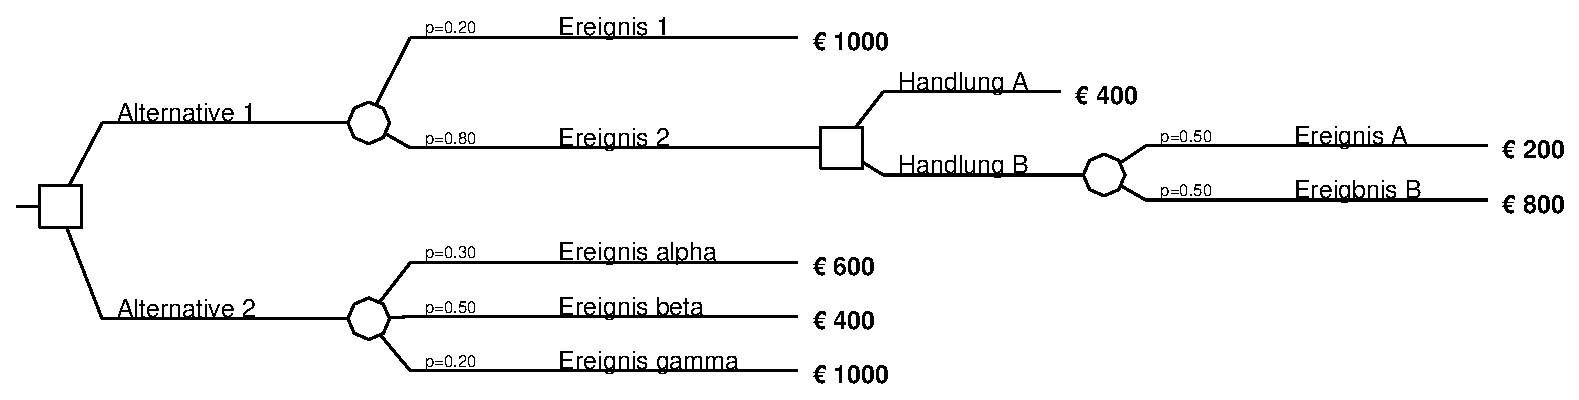
\includegraphics[width=22cm]{Grafiken/Klausur.eps}
\caption{Der Entscheidungsbaum zu Aufgabe \ref{BaumAufgabe}.}
\end{center}
\end{sidewaysfigure}
